\documentclass{beamer}
\usetheme{tokitex}

\usepackage{tikz}
\usepackage{graphics}
\usepackage{multirow}
\usepackage{tabto}
\usepackage{xspace}
\usepackage{amsmath}
\usepackage{hyperref}
\usepackage{wrapfig}
\usepackage{mathtools}

\usepackage{tikz}
\usepackage{clrscode3e}
\usepackage{gensymb}

\usepackage[english,bahasa]{babel}
\newtranslation[to=bahasa]{Section}{Bagian}
\newtranslation[to=bahasa]{Subsection}{Subbagian}

\usepackage{listings, lstautogobble}
\usepackage{color}

\definecolor{dkgreen}{rgb}{0,0.6,0}
\definecolor{gray}{rgb}{0.5,0.5,0.5}
\definecolor{mauve}{rgb}{0.58,0,0.82}

\lstset{frame=tb,
  language=c++,
  aboveskip=0mm,
  belowskip=0mm,
  showstringspaces=false,
  columns=fullflexible,
  keepspaces=true,
  basicstyle={\small\ttfamily},
  numbers=none,
  numberstyle=\tiny\color{gray},
  keywordstyle=\color{blue},
  commentstyle=\color{dkgreen},
  stringstyle=\color{mauve},
  breaklines=true,
  breakatwhitespace=true,
  lineskip={-3pt}
}

\usepackage{caption}
\captionsetup[figure]{labelformat=empty}

\newcommand{\progTerm}[1]{\textbf{#1}}
\newcommand{\foreignTerm}[1]{\textit{#1}}
\newcommand{\newTerm}[1]{\alert{\textbf{#1}}}
\newcommand{\emp}[1]{\alert{#1}}
\newcommand{\statement}[1]{"#1"}

\newcommand{\floor}[1]{\lfloor #1 \rfloor}
\newcommand{\ceil}[1]{\lceil #1 \rceil}
\newcommand{\abs}[1]{\left\lvert#1\right\rvert}
\newcommand{\norm}[1]{\left\lVert#1\right\rVert}

% Getting tired of writing \foreignTerm all the time
\newcommand{\farray}{\foreignTerm{array}\xspace}
\newcommand{\fArray}{\foreignTerm{Array}\xspace}
\newcommand{\foverhead}{\foreignTerm{overhead}\xspace}
\newcommand{\fOverhead}{\foreignTerm{Overhead}\xspace}
\newcommand{\fsubarray}{\foreignTerm{subarray}\xspace}
\newcommand{\fSubarray}{\foreignTerm{Subarray}\xspace}
\newcommand{\fbasecase}{\foreignTerm{base case}\xspace}
\newcommand{\fBasecase}{\foreignTerm{Base case}\xspace}
\newcommand{\ftopdown}{\foreignTerm{top-down}\xspace}
\newcommand{\fTopdown}{\foreignTerm{Top-down}\xspace}
\newcommand{\fbottomup}{\foreignTerm{bottom-up}\xspace}
\newcommand{\fBottomup}{\foreignTerm{Bottom-up}\xspace}
\newcommand{\fpruning}{\foreignTerm{pruning}\xspace}
\newcommand{\fPruning}{\foreignTerm{Pruning}\xspace}

\newcommand{\fgraph}{\foreignTerm{graph}\xspace}
\newcommand{\fGraph}{\foreignTerm{Graph}\xspace}
\newcommand{\froot}{\foreignTerm{root}\xspace}
\newcommand{\fRoot}{\foreignTerm{Root}\xspace}
\newcommand{\fnode}{\foreignTerm{node}\xspace}
\newcommand{\fNode}{\foreignTerm{Node}\xspace}
\newcommand{\fedge}{\foreignTerm{edge}\xspace}
\newcommand{\fEdge}{\foreignTerm{Edge}\xspace}
\newcommand{\fcycle}{\foreignTerm{cycle}\xspace}
\newcommand{\fCycle}{\foreignTerm{Cycle}\xspace}
\newcommand{\fdegree}{\foreignTerm{degree}\xspace}
\newcommand{\fDegree}{\foreignTerm{Degree}\xspace}
\newcommand{\fadjacencylist}{\foreignTerm{adjacency list}\xspace}
\newcommand{\fAdjacencylist}{\foreignTerm{Adjacency list}\xspace}
\newcommand{\fadjacencymatrix}{\foreignTerm{adjacency matrix}\xspace}
\newcommand{\fAdjacencymatrix}{\foreignTerm{Adjacency matrix}\xspace}
\newcommand{\fedgelist}{\foreignTerm{edge list}\xspace}
\newcommand{\fEdgelist}{\foreignTerm{Edge list}\xspace}
\newcommand{\flist}{\foreignTerm{list}\xspace}
\newcommand{\fList}{\foreignTerm{List}\xspace}
\newcommand{\fgraphtraversal}{\foreignTerm{graph traversal}\xspace}
\newcommand{\fGraphtraversal}{\foreignTerm{Graph traversal}\xspace}
\newcommand{\ftree}{\foreignTerm{tree}\xspace}
\newcommand{\fTree}{\foreignTerm{Tree}\xspace}
\newcommand{\fsubtree}{\foreignTerm{subtree}\xspace}
\newcommand{\fSubtree}{\foreignTerm{Subtree}\xspace}
\newcommand{\fparent}{\foreignTerm{parent}\xspace}
\newcommand{\fParent}{\foreignTerm{Parent}\xspace}
\newcommand{\fsibling}{\foreignTerm{sibling}\xspace}
\newcommand{\fSibling}{\foreignTerm{Sibling}\xspace}
\newcommand{\fpath}{\foreignTerm{path}\xspace}
\newcommand{\fPath}{\foreignTerm{Path}\xspace}
\newcommand{\fconnectedcomponent}{\foreignTerm{connected component}\xspace}
\newcommand{\fConnectedcomponent}{\foreignTerm{Connected component}\xspace}
\newcommand{\fbridge}{\foreignTerm{bridge}\xspace}
\newcommand{\fBridge}{\foreignTerm{Bridge}\xspace}
\newcommand{\farticulationpoint}{\foreignTerm{articulation point}\xspace}
\newcommand{\fArticulationpoint}{\foreignTerm{Articulation point}\xspace}
\newcommand{\ftreeedge}{\foreignTerm{tree edge}\xspace}
\newcommand{\fTreeedge}{\foreignTerm{Tree edge}\xspace}
\newcommand{\fbackedge}{\foreignTerm{back edge}\xspace}
\newcommand{\fBackedge}{\foreignTerm{Back edge}\xspace}
\newcommand{\fforwardedge}{\foreignTerm{forward edge}\xspace}
\newcommand{\fForwardedge}{\foreignTerm{Forward edge}\xspace}
\newcommand{\fcrossedge}{\foreignTerm{cross edge}\xspace}
\newcommand{\fCrossedge}{\foreignTerm{Cross edge}\xspace}
\newcommand{\fdiscoverytime}{\foreignTerm{discovery time}\xspace}
\newcommand{\fDiscoverytime}{\foreignTerm{Discovery time}\xspace}
\newcommand{\flowlink}{\foreignTerm{low link}\xspace}
\newcommand{\fLowlink}{\foreignTerm{Low link}\xspace}
\newcommand{\fstack}{\foreignTerm{stack}\xspace}
\newcommand{\fStack}{\foreignTerm{Stack}\xspace}
\newcommand{\for}{\foreignTerm{or}\xspace}
\newcommand{\fOr}{\foreignTerm{Or}\xspace}
\newcommand{\fand}{\foreignTerm{and}\xspace}
\newcommand{\fAnd}{\foreignTerm{And}\xspace}
\newcommand{\fcentroid}{\foreignTerm{centroid}\xspace}
\newcommand{\fCentroid}{\foreignTerm{Centroid}\xspace}

\newcommand{\fDivideAndConquer}{\foreignTerm{Divide and conquer}\xspace}
\newcommand{\fdivideAndConquer}{\foreignTerm{divide and conquer}\xspace}
\newcommand{\fMergeSort}{\foreignTerm{Merge sort}\xspace}
\newcommand{\fmergeSort}{\foreignTerm{merge sort}\xspace}
\newcommand{\fQuickSort}{\foreignTerm{Quicksort}\xspace}
\newcommand{\fquickSort}{\foreignTerm{quicksort}\xspace}
\newcommand{\fpivot}{\foreignTerm{pivot}\xspace}
\newcommand{\fPivot}{\foreignTerm{Pivot}\xspace}
\newcommand{\fbruteForce}{\foreignTerm{brute force}\xspace}
\newcommand{\fBruteForce}{\foreignTerm{Brute force}\xspace}
\newcommand{\fCompleteSearch}{\foreignTerm{complete search}\xspace}
\newcommand{\fExhaustiveSearch}{\foreignTerm{exhaustive search}\xspace}
\newcommand{\fbinarySearch}{\foreignTerm{binary search}\xspace}
\newcommand{\fBinarySearch}{\foreignTerm{Binary search}\xspace}
\newcommand{\fternarySearch}{\foreignTerm{ternary search}\xspace}
\newcommand{\fTernarySearch}{\foreignTerm{Ternary search}\xspace}
\newcommand{\funimodal}{\foreignTerm{unimodal}\xspace}
\newcommand{\fUnimodal}{\foreignTerm{Unimodal}\xspace}
\newcommand{\fGreedy}{\foreignTerm{Greedy}\xspace}
\newcommand{\fgreedy}{\foreignTerm{greedy}\xspace}
\newcommand{\fgreedyChoice}{\foreignTerm{greedy choice}\xspace}
\newcommand{\fGreedyChoice}{\foreignTerm{Greedy choice}\xspace}

\newcommand{\fdp}{\foreignTerm{dynamic programming}\xspace}
\newcommand{\fDp}{\foreignTerm{Dynamic programming}\xspace}
\newcommand{\fbitmask}{\foreignTerm{bitmask}\xspace}
\newcommand{\fBitmask}{\foreignTerm{Bitmask}\xspace}
\newcommand{\fstate}{\foreignTerm{state}\xspace}
\newcommand{\fState}{\foreignTerm{State}\xspace}
\newcommand{\fsubmask}{\foreignTerm{submask}\xspace}
\newcommand{\fSubmask}{\foreignTerm{Submask}\xspace}

\newcommand{\pheap}{\foreignTerm{heap}\xspace}
\newcommand{\pHeap}{\foreignTerm{Heap}\xspace}
\newcommand{\pBinaryHeap}{\foreignTerm{Binary Heap}\xspace}
\newcommand{\pbinaryHeap}{\foreignTerm{binary heap}\xspace}
\newcommand{\pHeapsort}{\foreignTerm{Heapsort}\xspace}
\newcommand{\pheapsort}{\foreignTerm{heapsort}\xspace}
\newcommand{\pdjs}{\foreignTerm{disjoint set}\xspace}
\newcommand{\pDjs}{\foreignTerm{Disjoint set}\xspace}

\newcommand{\fdotProduct}{\foreignTerm{dot product}\xspace}
\newcommand{\fDotProduct}{\foreignTerm{Dot product}\xspace}
\newcommand{\fcrossProduct}{\foreignTerm{cross product}\xspace}
\newcommand{\fCrossProduct}{\foreignTerm{Cross product}\xspace}
\newcommand{\fconvexHull}{\foreignTerm{convex hull}\xspace}
\newcommand{\fConvexHull}{\foreignTerm{Convex hull}\xspace}
\newcommand{\fgrahamScan}{\foreignTerm{graham scan}\xspace}
\newcommand{\fGrahamScan}{\foreignTerm{Graham scan}\xspace}
\newcommand{\flineSweep}{\foreignTerm{line sweep}\xspace}
\newcommand{\fLineSweep}{\foreignTerm{Line sweep}\xspace}

\newcommand{\fset}{\foreignTerm{set}\xspace}
\newcommand{\fSet}{\foreignTerm{Set}\xspace}
\newcommand{\fprefixSum}{\foreignTerm{prefix sum}\xspace}
\newcommand{\fPrefixSum}{\foreignTerm{Prefix sum}\xspace}
\newcommand{\ffenwickTree}{\foreignTerm{fenwick tree}\xspace}
\newcommand{\fFenwickTree}{\foreignTerm{Fenwick tree}\xspace}
\newcommand{\frangeSumQuery}{\foreignTerm{range sum query}\xspace}
\newcommand{\fRangeSumQuery}{\foreignTerm{Range sum query}\xspace}
\newcommand{\fquery}{\foreignTerm{query}\xspace}
\newcommand{\fQuery}{\foreignTerm{Query}\xspace}
\newcommand{\fsegmentTree}{\foreignTerm{segment tree}\xspace}
\newcommand{\fSegmentTree}{\foreignTerm{Segment tree}\xspace}
\newcommand{\fbinaryTree}{\foreignTerm{binary tree}\xspace}
\newcommand{\fBinaryTree}{\foreignTerm{Binary tree}\xspace}
\newcommand{\flazyPropagation}{\foreignTerm{lazy propagation}\xspace}
\newcommand{\fLazyPropagation}{\foreignTerm{Lazy propagation}\xspace}
\newcommand{\fsparseTable}{\foreignTerm{sparse table}\xspace}
\newcommand{\fSparseTable}{\foreignTerm{Sparse table}\xspace}

\newcommand{\ftrail}{\foreignTerm{trail}\xspace}
\newcommand{\fTrail}{\foreignTerm{Trail}\xspace}
\newcommand{\feulerTour}{\foreignTerm{euler tour}\xspace}
\newcommand{\fEulerTour}{\foreignTerm{Euler tour}\xspace}
\newcommand{\feulerTourTree}{\foreignTerm{euler tour tree}\xspace}
\newcommand{\fEulerTourTree}{\foreignTerm{Euler tour tree}\xspace}

\newcommand{\fmaxflow}{\foreignTerm{maximum flow}\xspace}
\newcommand{\fMaxflow}{\foreignTerm{Maximum flow}\xspace}
\newcommand{\fmincut}{\foreignTerm{minimum cut}\xspace}
\newcommand{\fMincut}{\foreignTerm{Minimum cut}\xspace}
\newcommand{\fflow}{\foreignTerm{flow}\xspace}
\newcommand{\fFlow}{\foreignTerm{Flow}\xspace}
\newcommand{\fsource}{\foreignTerm{source}\xspace}
\newcommand{\fSource}{\foreignTerm{Source}\xspace}
\newcommand{\fsink}{\foreignTerm{sink}\xspace}
\newcommand{\fSink}{\foreignTerm{Sink}\xspace}
\newcommand{\fbackEdge}{\foreignTerm{back-edge}\xspace}
\newcommand{\fBackEdge}{\foreignTerm{Back-edge}\xspace}
\newcommand{\fresidualCapacity}{\foreignTerm{residual capacity}\xspace}
\newcommand{\fResidualCapacity}{\foreignTerm{Residual capacity}\xspace}
\newcommand{\fbottleneck}{\foreignTerm{bottleneck}\xspace}
\newcommand{\fBottleneck}{\foreignTerm{Bottleneck}\xspace}
\newcommand{\faugmentingPath}{\foreignTerm{augmenting path}\xspace}
\newcommand{\fAugmentingPath}{\foreignTerm{Augmenting path}\xspace}


\title{Graf Lanjutan}
\author{Tim Olimpiade Komputer Indonesia}
\date{}

\usepackage{tikz} 

\begin{document}

\begin{frame}
\titlepage
\end{frame}

\begin{frame}
\frametitle{Pendahuluan}
Melalui dokumen ini, kalian akan:
\begin{itemize}
  \item Memahami Euler Tour Tree dan penggunaannya
  \item Memahami konsep Bridge, Articulation Point, dan Strongly Connected Component
  \item Memahami konsep Centroid Decomposition
\end{itemize}
\end{frame}

\begin{frame}
\frametitle{Euler Tour Tree}
\begin{itemize}
  \item \newTerm{Euler Tour} pada sebuah graf adalah sebuah \ftrail yang berawal di sebuah \fnode dan berakhir di \fnode yang sama dengan melalui setiap \fedge tepat satu kali.
  \item \newTerm{Euler Tour Tree} adalah salah satu cara mepresentasikan sebuah \ftree dengan mengasumsikan sebuah jalan yang awalnya tidak berarah menjadi dua buah jalan berarah bolak balik, dan mencari \feulerTour yang dimulai dari \froot.
\end{itemize}
\begin{figure}[!h]
\centering
  \begin{tikzpicture}[main/.style = {draw, circle}] 
  \node[main] (1) {};
  \node[main] (2) [below left of=1] {};
  \node[main] (3) [below left of=2] {};
  \node[main] (4) [below right of=2] {};
  \node[main] (5) [below of=4] {};
  \node[main] (6) [below right of=1] {};
  \draw[->] (1) -- (2);
  \draw[->] (2) -- (1);
  \draw[->] (2) -- (3);
  \draw[->] (3) -- (2);
  \draw[->] (2) -- (4);
  \draw[->] (4) -- (2);
  \draw[->] (4) -- (5);
  \draw[->] (5) -- (4);
  \draw[->] (1) -- (6);
  \draw[->] (6) -- (1);
  \end{tikzpicture}
\end{figure}
\end{frame}

\begin{frame}
\frametitle{Euler Tour Tree (lanj.)}
\begin{itemize}
  \item Jika kita menomori seluruh node sesuai dengan urutan \fnode yang dikunjungi pada \feulerTourTree, maka untuk setiap \fnode $u$, nomor-nomor seluruh \fnode yang berada pada \fsubtree \fnode $u$ berurutan.
  \item Sebagai contoh, nomor-nomor seluruh \fnode yang berada pada \fsubtree \fnode $2$ pada ilustrasi berikut adalah $\{2, 3, 4, 5\}$.
\end{itemize}
\begin{figure}[!h]
\centering
  \begin{tikzpicture}[main/.style = {draw, circle}] 
  \node[main] (1) {$1$}; 
  \node[main] (2) [below left of=1] {$2$};
  \node[main] (3) [below left of=2] {$3$}; 
  \node[main] (4) [below right of=2] {$4$};
  \node[main] (5) [below of=4] {$5$};
  \node[main] (6) [below right of=1] {$6$};
  \draw (1) -- (2);
  \draw (2) -- (3);
  \draw (2) -- (4);
  \draw (4) -- (5);
  \draw (1) -- (6);
  \end{tikzpicture}
\end{figure}
\end{frame}

\begin{frame}[fragile]
\frametitle{Euler Tour Tree (lanj.)}
\begin{itemize}
  \item Karena itu, jika setiap \fnode memiliki sebuah nilai, maka kita dapat menjumlahkan nilai seluruh \fnode yang berada pada \fsubtree sebuah \fnode menggunakan data struktur yang menyelesaikan persoalan \frangeSumQuery.
  \item Karena tidak terdapat \fcycle, menentukan urutan \fnode yang dikunjungi pada \feulerTourTree dapat diperoleh dengan DFS sederhana.
\end{itemize}
\begin{lstlisting}
// berisi pemetaan node ke urutan kunjungan
// pada euler tour tree.
map<Node, int> nomor;

void dfs(Node u, Node parent) {
  nomor[u] = nomor.size();
  for (Node v : u.neighbours()) {
    if (v != parent) {
      dfs(v, u);
    }
  }
}
\end{lstlisting}
\end{frame}

\begin{frame}
\frametitle{Graph Connectivity dalam graf tidak berarah}
\begin{itemize}
  \item Beberapa definisi dalam graf tidak berarah
  \begin{itemize}
    \item \newTerm{Connected component} adalah subgraf maksimal yang mana tiap dua vertexnya bisa dicapai satu sama lain melalui sebuah \fpath.
    \item Sebuah \fedge merupakan \newTerm{bridge} apabila jika edge tersebut dihapus maka banyaknya \fconnectedcomponent dari graf tersebut bertambah.
    \begin{itemize}
      \item Dengan kata lain, tidak terdapat \fpath lain yang menghubungkn dua \fnode yang merupakan ujung dari \fedge tersebut.
    \end{itemize}
    \item Sebuah \fnode merupakan \newTerm{articulation point} apabila jika \fnode tersebut dihapus maka banyaknya \fconnectedcomponent dari graf tersebut bertambah.
  \end{itemize}
\end{itemize}
\end{frame}

\begin{frame}
\frametitle{Graph Connectivity dalam graf tidak berarah (lanj.)}
\begin{itemize}
  \item Sebagai contoh, pada graf berikut, \fedge yang dicetak tebal merupakan \fbridge, sedangkan \fnode yang dicetak tebal merupakan \farticulationpoint.
\end{itemize}
\begin{figure}[!h]
\centering
  \begin{tikzpicture}[node distance=2cm, main/.style = {draw, circle}]
  \node[main, ultra thick] (2) {$2$};
  \node[main] (1) [above left of=2] {$1$};
  \node[main] (3) [below left of=2] {$3$};
  \node[main, ultra thick] (4) [below right of=2] {$4$};
  \node[main] (5) [above right of=4] {$5$};
  \node[main] (6) [above right of=2] {$6$};
  \node[main] (7) [right of=4] {$7$};
  \draw (1) -- (2);
  \draw (1) -- (3);
  \draw (2) -- (3);
  \draw (2) -- (4);
  \draw (4) -- (5);
  \draw (2) -- (6);
  \draw (5) -- (6);
  \draw[ultra thick] (4) -- (7);
  \end{tikzpicture}
\end{figure}
\end{frame}

\begin{frame}
\frametitle{Graph Connectivity dalam graf tidak berarah (lanj.)}
\begin{itemize}
  \item Pada sebuah graf tidak berarah:
  \begin{itemize}
    \item \newTerm{DFS Tree} dari graf tersebut adalah tree yang dihasilkan dari menjalankan algoritma DFS pada graf tersebut.
    \item Sebuah \fedge merupakan \newTerm{tree edge} jika \fedge tersebut berada pada DFS \ftree.
    \item Sebuah \fedge merupakan \newTerm{back edge} jika \fedge tersebut menghubungkan sebuah \fnode dengan leluhurnya.
    \begin{itemize}
      \item Perhatikan bahwa seluruh \fedge yang bukan merupakan \ftreeedge adalah \fbackedge.
    \end{itemize}
    \item \newTerm{Discovery time} dari sebuah \fnode adalah urutan node tersebut dikunjungi pada DFS.
    \item \newTerm{Low link} dari sebuah \fnode adalah \fdiscoverytime terkecil yang bisa dicapai oleh sebuah \fnode dengan \ftreeedge ke anak-anaknya dan \fbackedge paling banyak sekali.
  \end{itemize}
\end{itemize}
\end{frame}

\begin{frame}
\frametitle{Graph Connectivity dalam graf tidak berarah (lanj.)}
\begin{itemize}
  \item Sebagai contoh, ilustrasi berikut menunjukan DFS \ftree yang mungkin dihasilkan jika menjalankan algoritma DFS pada graf sebelumnya dimulai dengan \fnode $1$.
  \begin{itemize}
    \item \fedge yang dicetak tebal merupakan \ftreeedge, sedangkan yang tidak dicetak tebal merupakan \fbackedge
    \item Angka di dalam dan di luar \fnode menyatakan \fdiscoverytime dan \flowlink dari node tersebut secara berurutan.
  \end{itemize}
\end{itemize}
\begin{figure}[!h]
\centering
  \begin{tikzpicture}[node distance=1cm, main/.style = {draw, circle}]
  \node[main] (1) [label=right:1] {$1$};
  \node[main] (2) [label=right:1, below of=1] {$2$};
  \node[main] (3) [label=right:1, below left of=2] {$3$};
  \node[main] (4) [label=right:2, below right of=2] {$4$};
  \node[main] (5) [label=right:2, below left of=4] {$5$};
  \node[main] (6) [label=right:2, below left of=5] {$6$};
  \node[main] (7) [label=right:7, below right of=4] {$7$};
  \draw[ultra thick] (1) -- (2);
  \draw[ultra thick] (2) -- (3);
  \draw[ultra thick] (2) -- (4);
  \draw[ultra thick] (4) -- (5);
  \draw[ultra thick] (5) -- (6);
  \draw[ultra thick] (4) -- (7);
  \draw (1) -- (3);
  \draw (2) -- (6);
  \end{tikzpicture}
\end{figure}
\end{frame}

\begin{frame}
\frametitle{Bridge}
\begin{itemize}
  \item Mari kita notasikan \fdiscoverytime dan \flowlink dari \fnode $u$ sebagai $low(u)$ dan $num(u)$ secara berurutan.
  \item Sebuah \fbackedge tidak mungkin merupakan \fbridge, karena kedua \fnode yang merupakan ujung dari \fedge tersebut masih terhubung menggunakan \ftreeedge.
  \item Sebuah \ftreeedge yang menghubungkan \fnode $u$ dan $v$ (dengan \fnode $u$ merupakan \fparent dari \fnode $v$ pada DFS \ftree) merupakan \fbridge jika $low(v) > num(u)$.
  \begin{itemize}
    \item Jika $low(v) \le num(u)$, maka terdapat \fpath dari \fnode $v$ ke \fnode $u$ melalui \fbackedge tanpa melalui \fedge yang menghubungkan kedua \fnode tersebut.
  \end{itemize}
  \item Algoritma ini memiliki kompleksitas $O(V + E)$.
\end{itemize}
\end{frame}

\begin{frame}
\frametitle{Articulation point}
\begin{itemize}
  \item Jika sebuah edge menghubungkan \fnode $u$ dan $v$ (dengan \fnode $u$ merupakan \fparent dari \fnode $v$ pada DFS \ftree), $u$ bukan merupakan \froot dari DFS \ftree, dan $low(v) \ge num(u)$, maka \fnode $u$ merupakan \farticulationpoint.
  \begin{itemize}
    \item $low(v) \ge num(u)$ berarti menghapus \fnode $u$ menyebabkan \fnode $v$ tidak terhubung dengan \fparent dari \fnode $u$.
  \end{itemize}
  \item Untuk setiap \fnode $u$ yang bukan merupakan \froot, jika $low(v) < num(u)$ untuk semua \fnode $v$ yang merupakan anak dari \fnode $u$, maka \fnode $u$ bukan merupakan \farticulationpoint.
  \item \fRoot dari DFS \ftree merupakan \farticulationpoint jika dan hanya jika ia memiliki lebih dari satu anak.
  \item Algoritma ini memiliki kompleksitas $O(V + E)$.
\end{itemize}
\end{frame}

\begin{frame}[fragile]
\frametitle{Contoh kode}
\begin{itemize}
  \item Berikut ini adalah contoh kode untuk mencari seluruh \fbridge dan \farticulationpoint pada sebuah graf.
\end{itemize}
\begin{lstlisting}
void dfs(Node u, Node parent) {
  num[u] = low[u] = time++;
  for (Node v : adj[u]) {
    if (num[v] != UNDEFINED) {
      ++num_children[u];
      dfs(v, u);
      if (low[v] > num[u]) bridges.insert((u, v));
      if (low[v] >= num[u] && parent != UNDEFINED_NODE) {
        articulation_point.insert(u);
      }
      low[u] = min(low[u], low[v]);
    } else if (v != parent) {
      low[u] = min(low[u], num[v]);
    }
  }
}
\end{lstlisting}
\end{frame}

\begin{frame}[fragile]
\frametitle{Contoh kode (lanj.)}
\begin{itemize}
  \item Berikut ini adalah contoh kode untuk mencari seluruh \fbridge dan \farticulationpoint pada sebuah graf (lanj.).
\end{itemize}
\begin{lstlisting}
for (Node u : nodes) {
  if (num[u] == UNDEFINED) {
    dfs(u, UNDEFINED_NODE);
    if (num_children[u] > 1) {
      articulation_point.insert(root);
    }
  }
}
\end{lstlisting}
\end{frame}

\begin{frame}
\frametitle{Graph Connectivity dalam graf berarah}
\begin{itemize}
  \item Dalam graf berarah, \newTerm{strongly connected component} (SCC) adalah subgraf maksimal yang mana tiap dua vertexnya bisa dicapai satu sama lain melalui sebuah \fpath.
  \item Sebagai contoh, pada graf di bawah, kumpulan \fnode yang berada dalam satu daerah warna abu-abu merupakan SCC.
  \item Jika kita membuat graf berarah baru dengan membuat satu \fnode untuk setiap SCC dan menambahkan \fedge dari \fnode $u$ ke \fnode $v$ jika terdapat \fedge dari salah satu \fnode di SCC $u$ ke salah satu \fnode di SCC $v$, maka graf baru ini adalah sebuah DAG.
\end{itemize}
\begin{center}
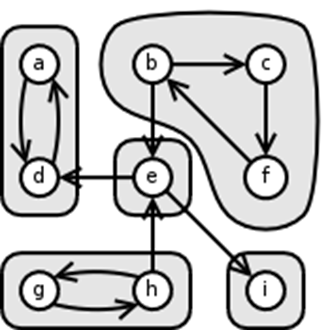
\includegraphics[width=3cm]{asset/scc.png}
\end{center}
\end{frame}

\begin{frame}
\frametitle{Algoritma Tarjan}
\begin{itemize}
  \item Untuk mencari seluruh SCC, kita dapat menggunakan algoritma Tarjan. Dapatkan DFS \ftree dari graf yang diberikan. Pada graf terarah, mungkin saja terdapat \fedge yang bukan merupakan \ftreeedge ataupun \fbackedge.
  \begin{itemize}
    \item Sebuah \fedge bisa saja merupakan \newTerm{forward edge}, yaitu \fedge yang berarah dari sebuah \fnode ke salah satu keturunannya. Untuk mencari SCC, \fedge ini dapat kita abaikan karena tidak mempengaruhi hasil SCC.
    \item Jika sebuah \fedge bukan merupakan \ftreeedge, \fbackedge, atau \fforwardedge, maka \fedge ini merupakan \newTerm{cross edge}. \fCrossedge pasti berarah dari sebuah \fnode yang memiliki \fdiscoverytime lebih tinggi ke sebuah \fnode yang memiliki \fdiscoverytime lebih rendah.
  \end{itemize}
\end{itemize}
\end{frame}

\begin{frame}
\frametitle{Algoritma Tarjan (lanj.)}
\begin{itemize}
  \item Apabila \fnode $u$ memiliki \fbackedge ke \fnode $v$, maka seluruh \fnode pada \fpath yang menghubungkan \fnode $u$ dan \fnode $v$ pada DFS \ftree pasti berada dalam satu SCC.
  \item Apabila \fnode $u$ memiliki \fcrossedge ke \fnode $v$, maka kita harus memeriksa apakah terdapat \fpath dari \fnode $v$ ke \fnode $u$ juga.
\end{itemize}
\end{frame}

\begin{frame}
\frametitle{Algoritma Tarjan (lanj.)}
\begin{itemize}
  \item Jalankan algoritma DFS. Pada akhir dari DFS di \fnode $u$, jika semua \fnode pada SCC yang berisi \fnode $u$ merupakan keturunan dari \fnode $u$, maka kita ingin membuat SCC tersebut.
  \begin{itemize}
    \item Untuk melakukan hal ini, sambil menjalankan algoritma DFS, kita ingin menjaga sebuah \fstack global $S$. Pada saat algoritma menjalakan DFS di \fnode $u$, $S$ berisi seluruh \fnode yang dapat mengunjungi \fnode $u$.
    \item Pada DFS di \fnode $u$, untuk setiap \fcrossedge dari \fnode $u$ ke \fnode $v$, jika \fnode $v$ berada pada stack $S$, maka kita dapat menganggap \fedge ini sebagai \fbackedge, sehingga kita dapat memperbaharui nilai $low(u)$ dengan $\min(low(u), num(v))$.
  \end{itemize}
\end{itemize}
\end{frame}

\begin{frame}
\frametitle{Algoritma Tarjan (lanj.)}
\begin{itemize}
  \item Jalankan algoritma DFS. Pada akhir dari DFS di \fnode $u$, jika semua \fnode pada SCC yang berisi \fnode $u$ merupakan keturunan dari \fnode $u$, maka kita ingin membuat SCC tersebut. (lanj.)
  \begin{itemize}
    \item Pada akhir DFS di \fnode $u$, jika $low(u) = num(u)$, ini berarti SCC yang berisi \fnode $u$ tidak berisi \fnode lain yang bukan merupakan keturunan \fnode $u$, sehingga kita dapat membuat sebuah SCC baru.
    \item Masukkan \fnode $u$ dan seluruh \fnode yang berada di atas \fnode $u$ pada stack $S$ ke dalam satu SCC baru, dan keluarkan seluruh \fnode tersebut dari $S$. Kumpulan \fnode ini adalah seluruh \fnode pada keturunan \fnode $u$ yang belum terdapat pada SCC manapun.
  \end{itemize}
  \item Algoritma ini memiliki kompleksitas $O(V + E)$.
\end{itemize}
\end{frame}

\begin{frame}[fragile]
\frametitle{Contoh kode}
\begin{itemize}
  \item Berikut ini adalah contoh kode untuk mencari seluruh SCC.
\end{itemize}
\begin{lstlisting}
void dfs(Node u) {
  num[u] = low[u] = time++;
  S.push(u); isInStack[u] = true;
  for (Node v : adj[u]) {
    if (num[v] != UNDEFINED) {
      dfs(v, u);
      low[u] = min(low[u], low[v]);
    } else if (isInStack[v]) {
      low[u] = min(low[u], num[v]);
    }
  }

  if (low[u] == num[u]) {
    set<Node> newScc;
    do {
      int s = stack.top(); scc.insert(s);
      stack.pop(); isInStack[s] = false;
    } while (s != u);
    sccs.insert(newScc);
  }
}
\end{lstlisting}
\end{frame}

\begin{frame}
\frametitle{Algoritma Kosaraju}
\begin{itemize}
  \item Selain algoritma Tarjan, kita juga dapat menggunakan algoritma Kosaraju untuk mendapatkan seluruh SCC.
  \item Algoritma Kosaraju juga memiliki kompleksitas $O(V + E)$.
  \item Kita tidak akan membahas algoritma Kosaraju pada pembelajaran ini.
\end{itemize}
\end{frame}

\begin{frame}
\frametitle{Contoh aplikasi: 2-SAT}
\begin{itemize}
  \item Persoalan 2-SAT adalah menentukan apakah ekspresi dalam bentuk konjungsi (\fand) dari beberapa klausa, dengan setiap klausa merupakan disjungsi (\for) dari dua literal, dapat bernilai benar. Setiap literal bisa saja merupakan suatu variabel atau negasi dari suatu variabel.
  \begin{itemize}
    \item Sebagai contoh, ekspresi $(x_2 \lor \neg x_1) \land (\neg x_2 \lor \neg x_1) \land (x_1 \lor x_3) \land (\neg x_2 \lor \neg x_3) \land (x_1 \lor x_4)$ dapat bernilai benar. Salah satu caranya dengan memberikan $x_1$ dan $x_2$ nilai salah dan memberikan $x_3$ dan $x_4$ nilai benar.
    \item Sebagai contoh lainnya, ekspresi $(x_1 \lor x_2) \land (x_1 \lor \neg x_2) \land (\neg x_1 \lor x_3) \land (\neg x_1 \lor \neg x_3)$ tidak dapat bernilai benar untuk seluruh kemungkinan pemberian nilai $x_1$, $x_2$, dan $x_3$.
  \end{itemize}
\end{itemize}
\end{frame}

\begin{frame}
\frametitle{Contoh aplikasi: Solusi 2-SAT}
\begin{itemize}
  \item Persoalan 2-SAT dapat diselesaikan dengan algoritma berikut:
  \begin{itemize}
    \item Buatlah sebuah graf baru $G$. Untuk setiap variabel $x$ pada ekspresi yang diberikan, tambahkan \fnode $x$ dan $\neg x$ pada $G$.
    \item Untuk setiap klausa $(a \lor b)$ (ekuivalen dengan $\neg a \Rightarrow b$ dan $\neg b \Rightarrow a$), tambahkan \fedge berarah dari \fnode $\neg a$ ke \fnode $b$ dan dari \fnode $\neg b$ ke \fnode $a$ pada $G$.
    \item Ekspresi yang diberikan dapat bernilai benar jika dan hanya jika kita dapat memberikan nilai salah/benar kepada setiap \fnode pada $G$ dengan syarat:
    \begin{itemize}
      \item \fnode $x$ dan \fnode $\neg x$ harus bernilai berbeda, dan
      \item untuk setiap \fedge dari \fnode $a$ ke \fnode $b$, jika \fnode $a$ bernilai benar, maka \fnode $b$ juga harus bernilai benar.
    \end{itemize}
    \item Jika terdapat sebuah SCC yang berisi \fnode $a$ dan \fnode $b$, maka kedua node ini harus bernilai sama. Karenanya, jika terdapat sebuah SCC yang berisi \fnode $x$ dan \fnode $\neg x$, maka ekspresi yang diberikan tidak dapat bernilai benar. Jika tidak, maka ekspresi yang diberikan dapat bernilai benar.
  \end{itemize}
\end{itemize}
\end{frame}

\begin{frame}
\frametitle{Centroid Decomposition}
\begin{itemize}
  \item Pada sebuah \ftree berisi $N$ \fnode, \newTerm{centroid} dari \ftree tersebut adalah sebuah \fnode yang jika \fnode tersebut dihapus, seluruh \ftree sisanya memiliki paling banyak $\frac{N}{2}$ \fnode. Mencari \fcentroid dapat dilakukan dalam kompleksitas $O(N)$.
  \item \newTerm{Centroid decomposition} (penguraian \fcentroid) adalah proses mencari \fcentroid pada sebuah tree, menghapus \fcentroid tersebut dari \ftree, lalu melakukan proses yang sama pada seluruh \ftree yang dihasilkan secara rekursif.
  \begin{itemize}
    \item Karena setiap penghapusan \fcentroid dari \ftree menyisakan \ftree yang memiliki \fnode paling banyak setengah dari banyak \fnode awal, proses rekursif ini memiliki kedalaman paling banyak $\lceil \log_2 N \rceil$.
    \item Untuk setiap tingkat kedalaman, jumlah banyaknya \fnode pada \ftree yang tersisa tidak lebih dari $N$. Sehingga, proses penguraian \fcentroid dapat dilakukan dalam kompleksitas $O(N \log N)$.
  \end{itemize}
\end{itemize}
\end{frame}

\begin{frame}
\frametitle{Centroid Decomposition: Contoh penggunaan}
\begin{itemize}
  \item Diberikan sebuah \ftree berbobot dan bilangan bulat $K$. Kita ingin menghitung berapa pasang \fnode yang dihubungkan oleh \fpath yang memiliki jarak (total bobot) tepat $K$.
  \item Persoalan ini dapat diselesaikan menggunakan penguraian \fcentroid:
  \begin{itemize}
    \item Misalkan \fnode $c$ adalah \fcentroid dari \ftree tersebut. Kita akan menghitung berapa pasang \fnode yang dihubungkan oleh \fpath yang melewati \fnode $c$ dan memiliki jarak $K$. Asumsikan menghapus \fnode $C$ menghasilkan dua \ftree terpisah $T_1$ dan $T_2$. Kita ingin menghitung berapa pasang \fnode $(a, b)$ sedemikian sehingga $a \in T_1$, $b \in T_2$, dan jumlah jarak \fnode $c$ dan \fnode $a$ dan jarak \fnode $c$ dan \fnode $b$ adalah $K$. Hal ini dapat dihitung dalam kompleksitas $O(N)$.
    \item Berikutnya, hapus \fnode $c$ dan lakukan algoritma ini secara rekursif pada seluruh \ftree yang tersisa untuk juga menghitung banyaknya pasang \fnode yang dihubungkan oleh \fpath yang tidak melewati \fnode $c$.
    \item Kompleksitas algoritma ini adalah $O(N \log N)$.
  \end{itemize}
\end{itemize}
\end{frame}

\end{document}
